\documentclass[a4paper]{article}

\usepackage[utf8]{inputenc}
\usepackage{erk}
\usepackage{times}
\usepackage{graphicx}
\usepackage[top=22.5mm, bottom=22.5mm, left=22.5mm, right=22.5mm]{geometry}

\usepackage[slovene,english]{babel}
\usepackage{hyperref}
\usepackage{url}
\usepackage{float}

\let\oldfootnotesize\footnotesize
\renewcommand*{\footnotesize}{\oldfootnotesize\scriptsize}

\begin{document}
\title{Navodila in osnutek prispevka za končno poročilo pri predmetu Računalniška grafika in tehnologija iger}

\author{Aljaž Kozina, Denis Kotnik, Kristian Žarn, Klemen Červ}

\affiliation{	Univerza v Ljubljani, Fakulteta za računalništvo in informatiko }

\email{E-pošta: kozinc@gmail.com, \\
 denis.kotnik@gmail.com, \\kristian.zarn@gmail.com, \\klemen.cerv@gmail.com}

\maketitle

\selectlanguage{slovene}

\begin{abstract}{Abstract}
V tretjeosebni pustolovščini vodiš ladjo, polno zaklada mimo nasprotnikov do pristanišča, medtem ko se trudiš, da bi izgubil čim manj zaklada.
\end{abstract}



\section{Pregled igre}
Naša igra je tretjeosebna pustolovščina, navdihnjena z igro Overboard!\cite{wiki:Overboard!}, v kateri igraš pirata, ki želi svoj zaklad prinesti v pristanišče, brez da bi mu ga drugi pirati ukradli ali potopili ladjo. Igra je lahke do srednje težavnosti, namenjena širši množici. V zaprtem svetu, oblikovanem kot labirint, se glavni igralec izogiba drugim ladjam ali pa jih napada s svojim orožjem medtem ko išče pristanišče.

\begin{figure}[H]
    \begin{center}
        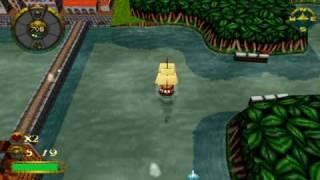
\includegraphics[width=\columnwidth]{Overboard.jpg}
        \caption{Navdih za našo igro.} \label{fig:slika}
    \end{center}
\end{figure}

\subsection{Opis sveta}
\textit{Na tem mestu podajte grob opis sveta v igri, ki ga podrobenje definirate v sledečih podpoglavjih. Prav tako definirajte v kakšnem stilu bo izdelan svet (npr. realističen, stiliziran, risankast, ipd.). Opredelite tudi ali se bodo osebki v svetu pomikali v eni, dveh ali treh dimenzijah.\\
}
\subsubsection{Pregled}
...

\subsubsection{Ozadje}
Ozadje sveta vsebuje nebo in kopno. Za nebo bodo predvidoma uporabljene javno dostopne teksture, za kopno pa predvidoma teksture in dodatni predmeti.

\subsubsection{Ključne lokacije}
V svetu so najbolj ključna lokacija pristanišča, kjer igralec išče ciljno pristanišče - tam lahko ladjo popravi in nadgrajuje, shrani zaklad in dobi novo ciljno pristanišče. Druge pomembne lokacije so nahajališča dobrin, kjer lahko igralec pobere dodaten zaklad ali pa si popravi ladjo, ter druga pristanišča, kamor se igralec lahko vrne s delom preostalega zakladom, če mu nasprotniki uničejo ladjo, kamor pa ne more shraniti zaklada.

\subsubsection{Velikost}
Svet je velikosti neke pokrajine in je sestavljen iz kopna in morja. Igralec z ladjo pluje po morju, kopno pa je ovira in omejuje njegovo gibanje. Svet je velik, a vendar omejen. Igralec bo postavljen na naključno lokacijo v svetu, prebiti pa se mora do pravega pristanišča. 

\subsubsection{Objekti}
Poglavitni objekti, ki bodo zajeti v igri, bodo ladje - igralčeva in nasprotnikove, pokrajina, sestavljena iz prednarejenih kosov in ključne lokacije, kot na primer pristanišče, ki jih bo izdelal naš grafični oblikovalec.

\subsubsection{Čas}
Igralec ladjo premika v realnem času, premikanje ladje pa je pospešeno v primerjavi z realnim časom zaradi povečane odzivnosti. Ker igra ni razdeljena na obdobja, čas v igri nima igralnega pomena.

\subsection{Igralni pogon in uporabljene tehnologije}
Pri izdelavi našega seminarja bomo v prvem delu predvidoma uporabili WebGL, Three.js \cite{dirksen2013learning}, Bullet.js ipd., v drugem delu pa se bomo obrnili na Unity.

\subsection{Pogled}
Pogled v našo igro bo omogočen na dva načina, med katerimi bo mogoče prosto menjati:
\begin{enumerate}
\item Pogled izza ladje - kamera bo vezana na zadnji del ladje in bo lokacijo in smer/rotacijo spreminjala skupaj z ladjo
\item Pogled od zgoraj - kamera bo na ladjo gledala od zgoraj navzdol, z nagibom in bo na ladjo vezana le z lokacijo, smer in rotacija bo statična, naklon kamere pa bo lahko nadzoroval uporabnik (Slika \ref{fig:slika})
\end{enumerate}


\small
\bibliographystyle{ieeetr}
\bibliography{references}

\end{document}
